% Inbuilt themes in beamer
\documentclass[aspectratio=169]{beamer}
\usepackage{graphicx}
% Theme choice:
\usetheme{CambridgeUS}

% Title page details: 
\title{Chapter 13: Costs of Production} 
\author{Discussion section 4}
\date{Feb 2024}

\begin{document}

% Title page
\begin{frame}
    \titlepage 
\end{frame}

% Outline frame
\begin{frame}{Outline}
    \begin{itemize}
        \item From Mankiw himself: this material is ``technical'' and even ``boring''.
        \item But, really important if we want to understand firms' decision making!
        \item Ch. 13 introduces us to the difference between \textit{economic} and \textit{accounting} costs and profits.
        \item We will then explore about different kinds of costs and how they may vary based on output and time scale.
    \end{itemize}
\end{frame}

\begin{frame}{Firms' Goal}
    \begin{itemize}
        \item Total revenue is all the money coming in.
            \begin{itemize}
                \item TR = P*Q
            \end{itemize}
        \item Total cost is the total \textit{opportunity cost} faced by a firm
            \begin{itemize}
                \item \textit{Economic} costs include explicit and implicit costs
                \item Different from \textit{accounting} costs which only include explicit costs
                \item Firms (and economists) are interested in the economic costs
            \end{itemize}
        \item Firms maximize total profits
            \begin{itemize}
                \item Total profit = TR - TC
            \end{itemize}
    \end{itemize}
\end{frame}

\begin{frame}{Example}
    \begin{itemize}
        \item Consider a bike shop which sells and repairs bicycles.
        \item What are some of the shop's \textit{accounting} costs?
        \item What are some of the shop's \textit{economic} costs?
    \end{itemize}
\end{frame}

\begin{frame}{Example}
    \begin{itemize}
        \item Consider a bike shop which sells and repairs bicycles.
        \item What are some of the shop's \textit{accounting} costs?
            \begin{itemize}
                \item Wages and benefits for workers
                \item Cost of supplies for bike repairs
                \item Rent/mortgage/upkeep on the store space
            \end{itemize}
        \item What are some of the shop's \textit{economic} costs?
            \begin{itemize}
                \item Revenue they could get from renting out bikes instead of selling them
                \item Interest they could earn if they put their money in a bond instead
            \end{itemize}
    \end{itemize}
\end{frame}

\begin{frame}{Example}
    \begin{itemize}
        \item Usually, we assume that in the short run capital is fixed and other inputs are variable.
        \item What capital does the bike shop have?
        \item Which costs mentioned before might be variable in the long run?
    \end{itemize}
\end{frame}

\begin{frame}{Example}
    \begin{itemize}
        \item Usually, we assume that in the short run capital is fixed and other inputs are variable.
        \item What capital does the bike shop have?
            \begin{itemize}
                \item The store/repair space
                \item Repair equipment
            \end{itemize}
        \item Which costs mentioned before might be variable in the long run?
            \begin{itemize}
                \item Rent/mortgage
                \item Wages for workers
            \end{itemize}
    \end{itemize}
\end{frame}

\begin{frame}{Production function}
    \begin{itemize}
        \item The production function tells us how much output a firm is able to produce with a given level of inputs
        \item Let's us derive the \textit{marginal product} of an input: how much does output change from a ``small'' (1 unit) increase in an input?
        \item This is usually not linear, so that marginal product is different at different levels of input.
        \item At some point, most inputs exhibit \textit{diminishing marginal product}: each additional unit of input increases output by less than the previous input.
    \end{itemize}
\end{frame}

\begin{frame}{Diminishing marginal product of labor}
    \centering
    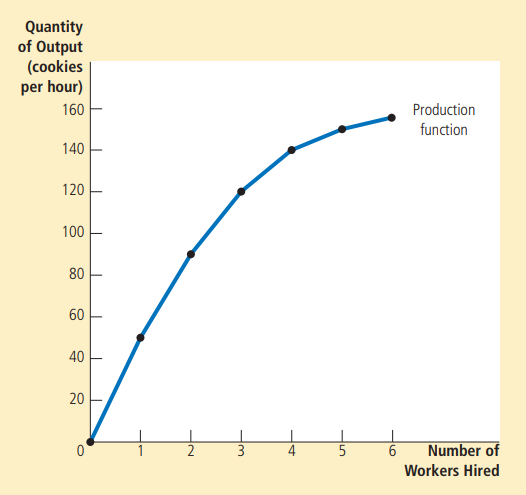
\includegraphics[width = 0.5\textwidth,keepaspectratio]{diminishingMPL.png}
\end{frame}

\begin{frame}{Total costs}
    If marginal product is decreasing, what happens to total costs as output goes up?
\end{frame}

\begin{frame}{Diminishing marginal product of labor}
    \centering
    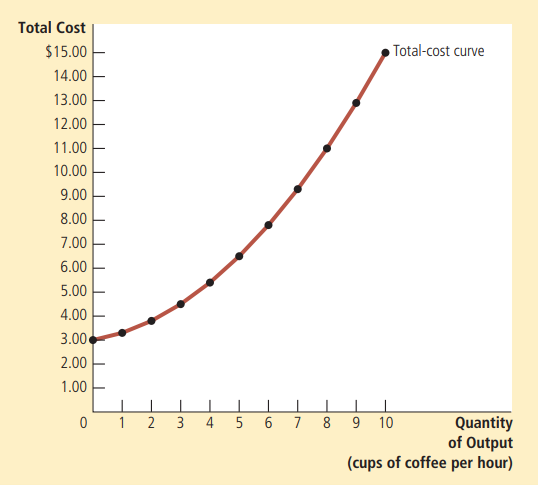
\includegraphics[width = 0.5\textwidth,keepaspectratio]{increasingTC.png}
\end{frame}

\begin{frame}{Fixed v. variable costs}
    \begin{itemize}
        \item Fixed costs are the same no matter how much output the firm produces
        \item Variable costs depend on the level of our output
        \item In our bike shop example, what are some fixed costs?
        \item What are some variable costs?
    \end{itemize}
\end{frame}

\begin{frame}{Fixed v. variable costs}
    \begin{itemize}
        \item Fixed costs are the same no matter how much output the firm produces
        \item Variable costs depend on the level of our output
        \item In our bike shop example, what are some fixed costs?
            \begin{itemize}
                \item Rent, ad campaign
            \end{itemize}
        \item What are some variable costs?
            \begin{itemize}
                \item Wages, bike tubes, etc.
            \end{itemize}
        \item Again, time period is important! Fixed costs may be variable in the long run.
    \end{itemize}
\end{frame}

\begin{frame}{Average costs}
    \begin{itemize}
        \item Average cost = TC / output
        \item Average fixed cost is always decreasing, while average variable costs may decrease or increase
        \item Marginal cost is the change in total cost from a ``small'' (1 unit) increase in output
        \item If marginal product is decreasing, what happens to marginal cost?
    \end{itemize}
\end{frame}

\begin{frame}{Marginal costs}
    \begin{itemize}
        \item If marginal product is decreasing, what happens to marginal cost?
            \begin{itemize}
                \item Marginal cost is increasing: each additional unit of output is occuring using a larger amount of inputs than before
            \end{itemize}
        \item If marginal costs are increasing, what happens to the average total cost?
    \end{itemize}
\end{frame}

\begin{frame}{U-shaped total costs}
    \centering
    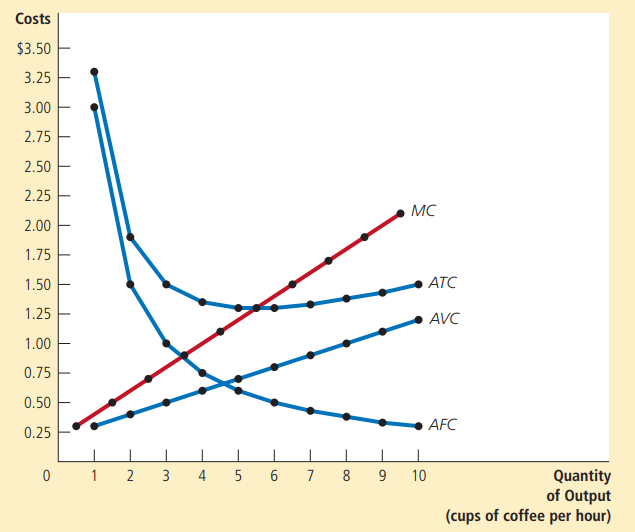
\includegraphics[width = 0.5\textwidth,keepaspectratio]{uTC.png}
\end{frame}

\begin{frame}{Marginal costs}
    \begin{itemize}
        \item If marginal costs are increasing, what happens to the average total cost?
            \begin{itemize}
                \item ATC decreases when ATC $>$ MC and increases once MC $>$ ATC
            \end{itemize}
        \item This means the MC curve crosses the ATC curve at the \textit{minimum} of ATC
    \end{itemize}
\end{frame}

\begin{frame}{Increasing marginal product}
    \begin{itemize}
        \item Marginal product is \textit{not} always decreasing
            \begin{itemize}
                \item Particularly true early in production process
            \end{itemize}
        \item This means that marginal cost is also \textit{not} always increasing
    \end{itemize}
\end{frame}

\begin{frame}{Decreasing MC}
    \centering
    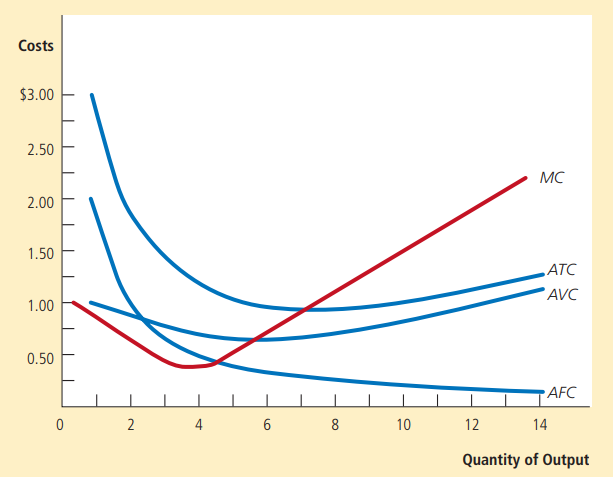
\includegraphics[width = 0.5\textwidth,keepaspectratio]{decreasingMC.png}
\end{frame}

\begin{frame}{Short- vs. long-run}
    \begin{itemize}
        \item Costs may be different in the short and long run!
            \begin{itemize}
                \item Economies of scale: long-run ATC decreases as output increases
                \item Diseconomies of scale: long-run ATC increases as output increases
                \item Constant returns scale: long-run ATC unchanged as output increases 
            \end{itemize}
        \item Why might we have economies of scale?
    \end{itemize}
\end{frame}

\begin{frame}{Short- vs. long-run}
    \begin{itemize}
        \item Why might we have economies of scale?
            \begin{itemize}
                \item specialization
                \item organization
                \item Purchasing power
            \end{itemize}
    \end{itemize}
\end{frame}

\begin{frame}{Decreasing MC}
    \centering
    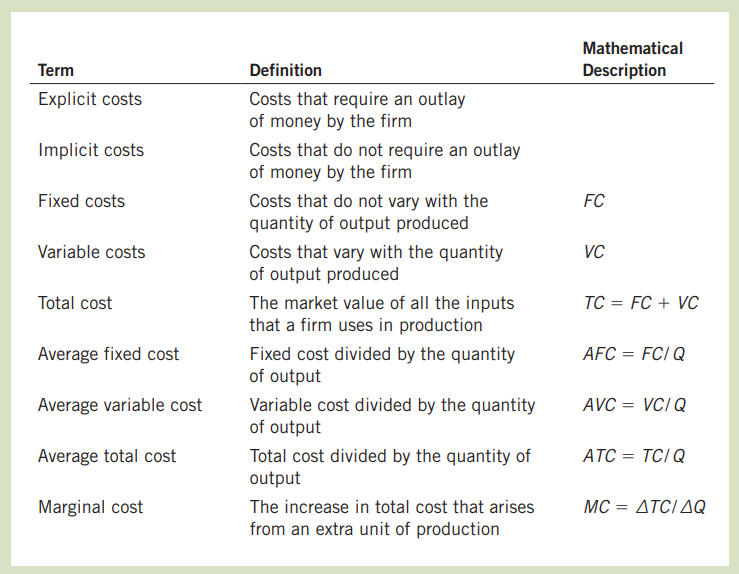
\includegraphics[width = 0.5\textwidth,keepaspectratio]{summary.png}
\end{frame}

% Costs which are fixed in the short run are variable in the long run; so long run cost curves are different from short run cost curves
% Economies of scale: long-run ATC decreases as output increases
% Diseconomies of scale -- long-run ATC increases
% constant economices of scale -- no change to ATC
% related to specialization, organization 
% Summary table

\end{document}
